% Généré par ./bin/gantt à partir de : results/exp_real_all/tasks/rr_r1.csv results/exp_real_all/tasks/select-maxmin_r1.csv
% Durées MESURÉES par l'orchestrateur (start_s / end_s).
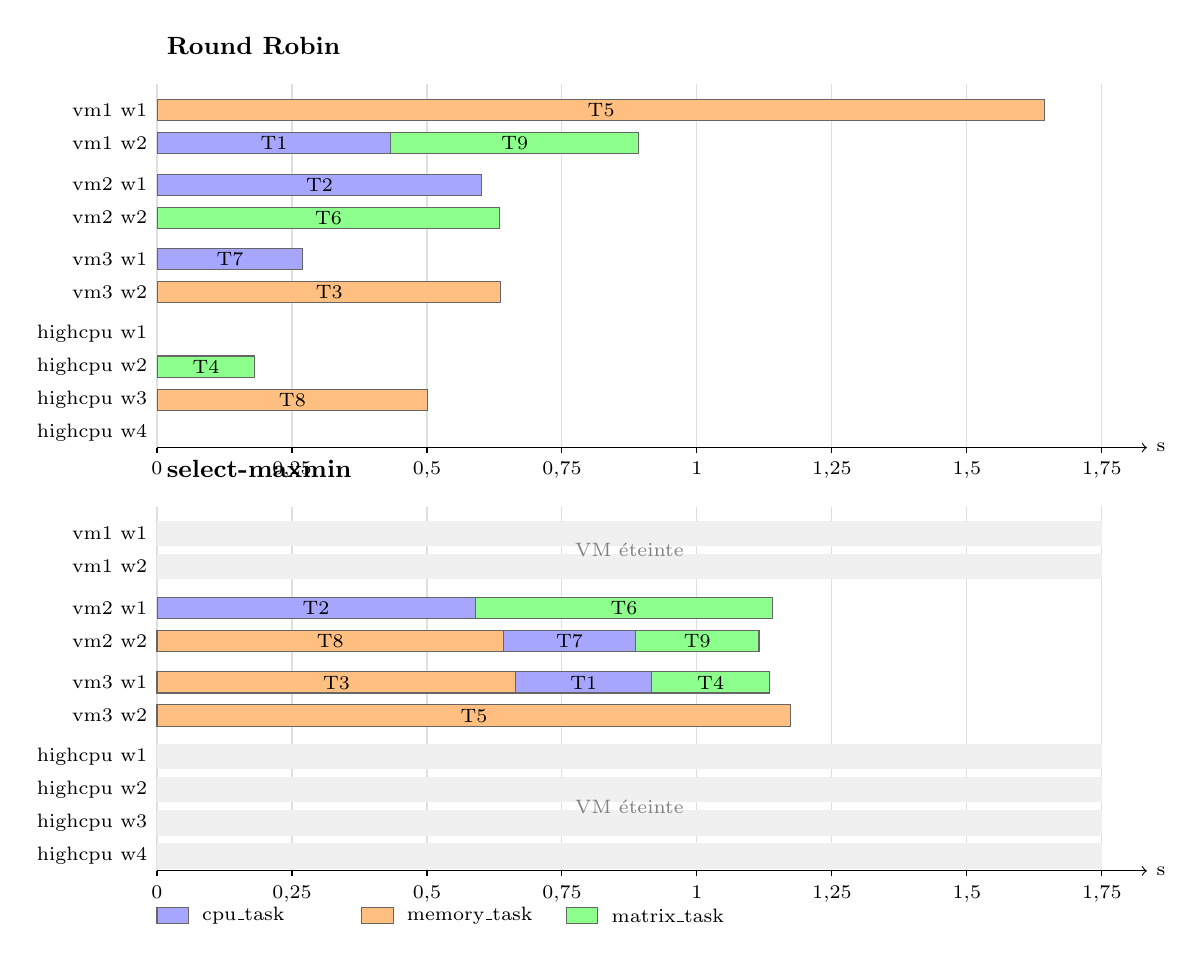
\begin{tikzpicture}[x=6.8571cm, y=0.42cm, font=\scriptsize]
  \node[anchor=south west, font=\small\bfseries] at (0,0.40) {Round Robin};
  \draw[gray!25] (0.0000,-11.20) -- (0.0000,-0.20);
  \draw[gray!25] (0.2500,-11.20) -- (0.2500,-0.20);
  \draw[gray!25] (0.5000,-11.20) -- (0.5000,-0.20);
  \draw[gray!25] (0.7500,-11.20) -- (0.7500,-0.20);
  \draw[gray!25] (1.0000,-11.20) -- (1.0000,-0.20);
  \draw[gray!25] (1.2500,-11.20) -- (1.2500,-0.20);
  \draw[gray!25] (1.5000,-11.20) -- (1.5000,-0.20);
  \draw[gray!25] (1.7500,-11.20) -- (1.7500,-0.20);
  \node[anchor=east] at (0,-1.00) {vm1 w1};
  \node[anchor=east] at (0,-2.00) {vm1 w2};
  \node[anchor=east] at (0,-3.25) {vm2 w1};
  \node[anchor=east] at (0,-4.25) {vm2 w2};
  \node[anchor=east] at (0,-5.50) {vm3 w1};
  \node[anchor=east] at (0,-6.50) {vm3 w2};
  \node[anchor=east] at (0,-7.75) {highcpu w1};
  \node[anchor=east] at (0,-8.75) {highcpu w2};
  \node[anchor=east] at (0,-9.75) {highcpu w3};
  \node[anchor=east] at (0,-10.75) {highcpu w4};
  \draw[fill=green!45, draw=black!60] (0.0002,-9.07) rectangle (0.1814,-8.43);
  \node at (0.0908,-8.75) {T4};
  \draw[fill=orange!50, draw=black!60] (0.0005,-10.07) rectangle (0.5011,-9.43);
  \node at (0.2508,-9.75) {T8};
  \draw[fill=blue!35, draw=black!60] (0.0008,-3.57) rectangle (0.6016,-2.93);
  \node at (0.3012,-3.25) {T2};
  \draw[fill=blue!35, draw=black!60] (0.0008,-2.32) rectangle (0.4330,-1.68);
  \node at (0.2169,-2.00) {T1};
  \draw[fill=orange!50, draw=black!60] (0.0008,-1.32) rectangle (1.6443,-0.68);
  \node at (0.8226,-1.00) {T5};
  \draw[fill=orange!50, draw=black!60] (0.0009,-6.82) rectangle (0.6370,-6.18);
  \node at (0.3190,-6.50) {T3};
  \draw[fill=green!45, draw=black!60] (0.0010,-4.57) rectangle (0.6341,-3.93);
  \node at (0.3176,-4.25) {T6};
  \draw[fill=blue!35, draw=black!60] (0.0012,-5.82) rectangle (0.2690,-5.18);
  \node at (0.1351,-5.50) {T7};
  \draw[fill=green!45, draw=black!60] (0.4331,-2.32) rectangle (0.8921,-1.68);
  \node at (0.6626,-2.00) {T9};
  \draw[->] (0,-11.20) -- (1.8333,-11.20) node[right] {s};
  \draw (0.0000,-11.20) -- (0.0000,-11.35) node[below] {0};
  \draw (0.2500,-11.20) -- (0.2500,-11.35) node[below] {0{,}25};
  \draw (0.5000,-11.20) -- (0.5000,-11.35) node[below] {0{,}5};
  \draw (0.7500,-11.20) -- (0.7500,-11.35) node[below] {0{,}75};
  \draw (1.0000,-11.20) -- (1.0000,-11.35) node[below] {1};
  \draw (1.2500,-11.20) -- (1.2500,-11.35) node[below] {1{,}25};
  \draw (1.5000,-11.20) -- (1.5000,-11.35) node[below] {1{,}5};
  \draw (1.7500,-11.20) -- (1.7500,-11.35) node[below] {1{,}75};
  \node[anchor=south west, font=\small\bfseries] at (0,-12.40) {select-maxmin};
  \draw[gray!25] (0.0000,-24.00) -- (0.0000,-13.00);
  \draw[gray!25] (0.2500,-24.00) -- (0.2500,-13.00);
  \draw[gray!25] (0.5000,-24.00) -- (0.5000,-13.00);
  \draw[gray!25] (0.7500,-24.00) -- (0.7500,-13.00);
  \draw[gray!25] (1.0000,-24.00) -- (1.0000,-13.00);
  \draw[gray!25] (1.2500,-24.00) -- (1.2500,-13.00);
  \draw[gray!25] (1.5000,-24.00) -- (1.5000,-13.00);
  \draw[gray!25] (1.7500,-24.00) -- (1.7500,-13.00);
  \node[anchor=east] at (0,-13.80) {vm1 w1};
  \fill[gray!12] (0,-14.18) rectangle (1.7500,-13.42);
  \node[anchor=east] at (0,-14.80) {vm1 w2};
  \fill[gray!12] (0,-15.18) rectangle (1.7500,-14.42);
  \node[gray] at (0.8750,-14.30) {VM éteinte};
  \node[anchor=east] at (0,-16.05) {vm2 w1};
  \node[anchor=east] at (0,-17.05) {vm2 w2};
  \node[anchor=east] at (0,-18.30) {vm3 w1};
  \node[anchor=east] at (0,-19.30) {vm3 w2};
  \node[anchor=east] at (0,-20.55) {highcpu w1};
  \fill[gray!12] (0,-20.93) rectangle (1.7500,-20.17);
  \node[anchor=east] at (0,-21.55) {highcpu w2};
  \fill[gray!12] (0,-21.93) rectangle (1.7500,-21.17);
  \node[anchor=east] at (0,-22.55) {highcpu w3};
  \fill[gray!12] (0,-22.93) rectangle (1.7500,-22.17);
  \node[anchor=east] at (0,-23.55) {highcpu w4};
  \fill[gray!12] (0,-23.93) rectangle (1.7500,-23.17);
  \node[gray] at (0.8750,-22.05) {VM éteinte};
  \draw[fill=orange!50, draw=black!60] (0.0001,-19.62) rectangle (1.1738,-18.98);
  \node at (0.5870,-19.30) {T5};
  \draw[fill=orange!50, draw=black!60] (0.0001,-17.37) rectangle (0.6416,-16.73);
  \node at (0.3209,-17.05) {T8};
  \draw[fill=orange!50, draw=black!60] (0.0001,-18.62) rectangle (0.6646,-17.98);
  \node at (0.3324,-18.30) {T3};
  \draw[fill=blue!35, draw=black!60] (0.0002,-16.37) rectangle (0.5891,-15.73);
  \node at (0.2946,-16.05) {T2};
  \draw[fill=green!45, draw=black!60] (0.5892,-16.37) rectangle (1.1406,-15.73);
  \node at (0.8649,-16.05) {T6};
  \draw[fill=blue!35, draw=black!60] (0.6417,-17.37) rectangle (0.8861,-16.73);
  \node at (0.7639,-17.05) {T7};
  \draw[fill=blue!35, draw=black!60] (0.6647,-18.62) rectangle (0.9160,-17.98);
  \node at (0.7903,-18.30) {T1};
  \draw[fill=green!45, draw=black!60] (0.8862,-17.37) rectangle (1.1150,-16.73);
  \node at (1.0006,-17.05) {T9};
  \draw[fill=green!45, draw=black!60] (0.9160,-18.62) rectangle (1.1348,-17.98);
  \node at (1.0254,-18.30) {T4};
  \draw[->] (0,-24.00) -- (1.8333,-24.00) node[right] {s};
  \draw (0.0000,-24.00) -- (0.0000,-24.15) node[below] {0};
  \draw (0.2500,-24.00) -- (0.2500,-24.15) node[below] {0{,}25};
  \draw (0.5000,-24.00) -- (0.5000,-24.15) node[below] {0{,}5};
  \draw (0.7500,-24.00) -- (0.7500,-24.15) node[below] {0{,}75};
  \draw (1.0000,-24.00) -- (1.0000,-24.15) node[below] {1};
  \draw (1.2500,-24.00) -- (1.2500,-24.15) node[below] {1{,}25};
  \draw (1.5000,-24.00) -- (1.5000,-24.15) node[below] {1{,}5};
  \draw (1.7500,-24.00) -- (1.7500,-24.15) node[below] {1{,}75};
  \draw[fill=blue!35, draw=black!60] (0.0000,-25.60) rectangle ++(0.0583,0.5);
  \node[anchor=west] at (0.0656,-25.35) {cpu\_task};
  \draw[fill=orange!50, draw=black!60] (0.3792,-25.60) rectangle ++(0.0583,0.5);
  \node[anchor=west] at (0.4448,-25.35) {memory\_task};
  \draw[fill=green!45, draw=black!60] (0.7583,-25.60) rectangle ++(0.0583,0.5);
  \node[anchor=west] at (0.8240,-25.35) {matrix\_task};
\end{tikzpicture}
